\documentclass[border=4pt]{standalone}
\usepackage{tikz}
\usepackage{amsmath,amssymb}
\usepackage{lmodern}
\renewcommand{\familydefault}{\sfdefault}
\usetikzlibrary{shapes.geometric,arrows.meta,positioning,calc,fit,backgrounds}

\begin{document}
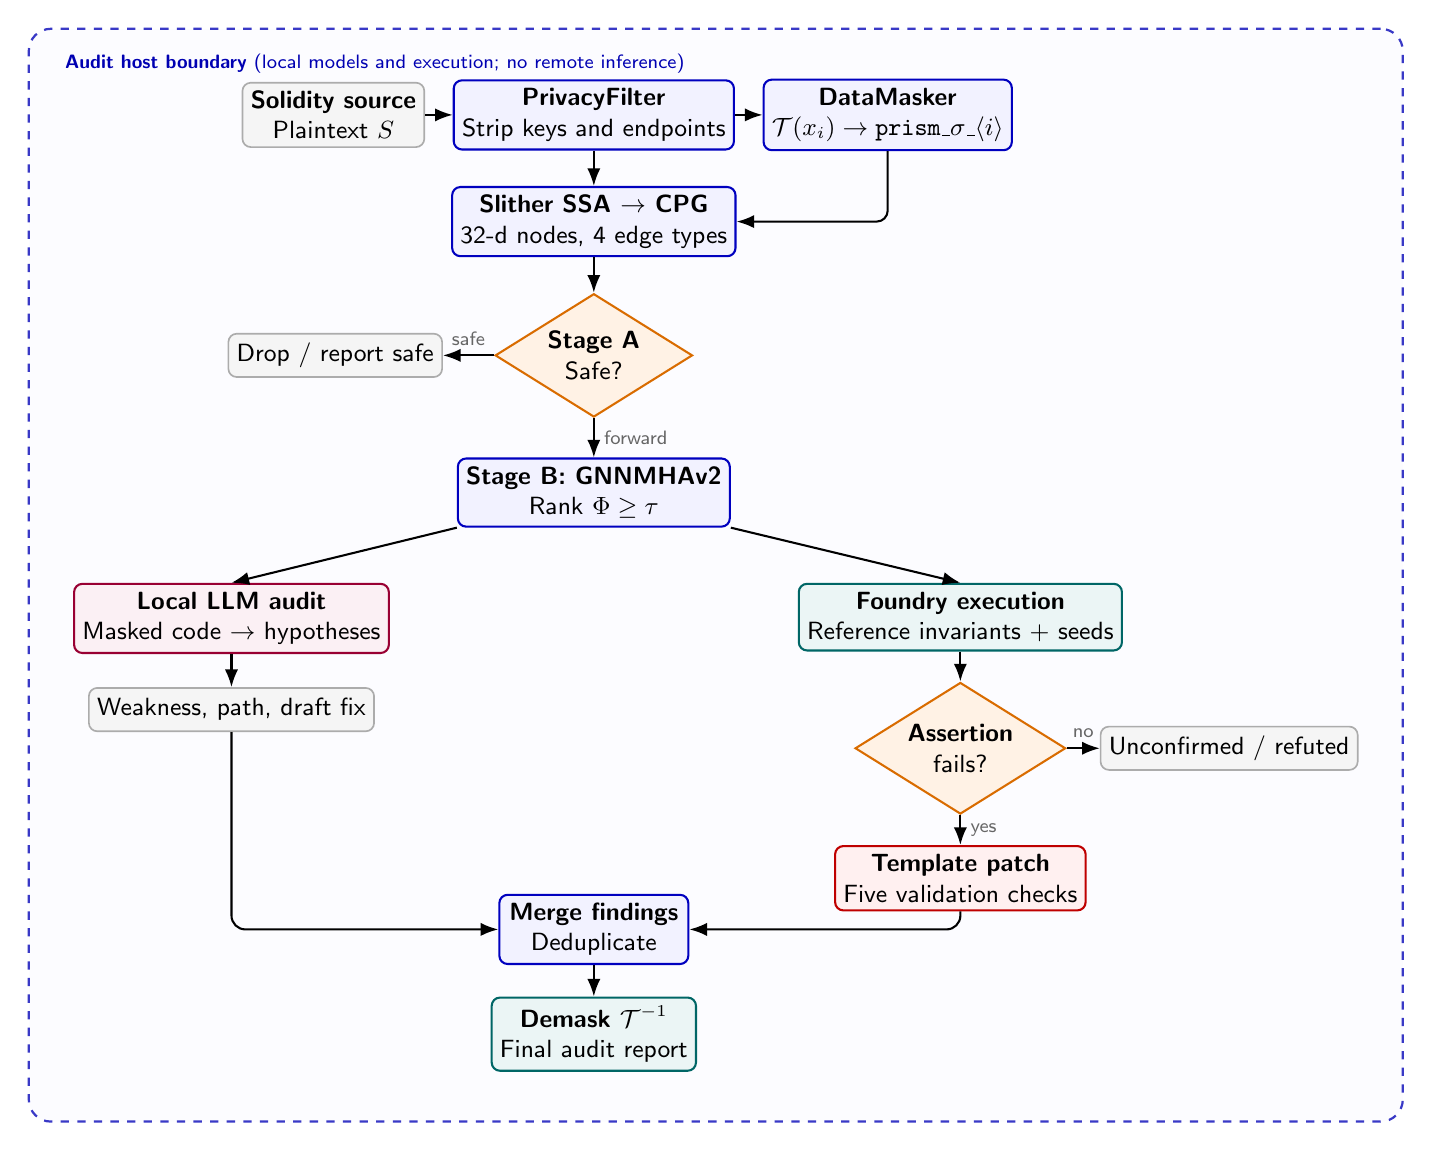
\begin{tikzpicture}[
  font=\sffamily\small,
  >=Latex,
  every node/.style={align=center},
  block/.style={rectangle, draw=blue!75!black, fill=blue!5, rounded corners=3pt, minimum height=0.68cm, minimum width=2.3cm, inner sep=3pt, line width=0.75pt},
  gate/.style={diamond, aspect=1.6, draw=orange!85!black, fill=orange!10, minimum width=1.6cm, inner sep=2pt, line width=0.75pt},
  action/.style={rectangle, draw=teal!80!black, fill=teal!8, rounded corners=3pt, minimum height=0.68cm, minimum width=2.35cm, inner sep=3pt, line width=0.75pt},
  llmblock/.style={rectangle, draw=purple!80!black, fill=purple!6, rounded corners=3pt, minimum height=0.68cm, minimum width=2.35cm, inner sep=3pt, line width=0.75pt},
  leaf/.style={rectangle, draw=gray!65, fill=gray!8, rounded corners=3pt, minimum height=0.55cm, minimum width=1.9cm, inner sep=3pt, line width=0.6pt},
  patch/.style={rectangle, draw=red!75!black, fill=red!6, rounded corners=3pt, minimum height=0.68cm, minimum width=2.2cm, inner sep=3pt, line width=0.75pt},
  subtle/.style={font=\sffamily\scriptsize, text=gray!80!black}
]

  % Confidential preprocessing (Top row)
  \node[leaf] (src) {\textbf{Solidity source}\\Plaintext $S$};
  \node[block, right=0.35cm of src] (pf) {\textbf{PrivacyFilter}\\Strip keys and endpoints};
  \node[block, right=0.35cm of pf] (dm) {\textbf{DataMasker}\\$\mathcal{T}(x_i)\to\texttt{prism\_}\sigma\_\langle i\rangle$};
  \node[block, below=0.45cm of pf] (cpg) {\textbf{Slither SSA $\to$ CPG}\\32-d nodes, 4 edge types};

  % Screening (Center column)
  \node[gate, below=0.45cm of cpg] (stgA) {\textbf{Stage A}\\Safe?};
  \node[leaf, left=0.65cm of stgA] (safe) {Drop / report safe};
  \node[block, below=0.5cm of stgA] (stgB) {\textbf{Stage B: GNNMHAv2}\\Rank $\Phi\ge\tau$};

  % Parallel hypothesis and execution stages (Symmetric left/right columns)
  \node[llmblock, below left=0.7cm and 0.85cm of stgB] (llm) {\textbf{Local LLM audit}\\Masked code $\to$ hypotheses};
  \node[action, below right=0.7cm and 0.85cm of stgB] (fuzz) {\textbf{Foundry execution}\\Reference invariants + seeds};

  \node[leaf, below=0.42cm of llm] (hyp) {Weakness, path, draft fix};

  \node[gate, below=0.38cm of fuzz] (cex) {\textbf{Assertion}\\fails?};
  \node[leaf, right=0.42cm of cex] (unconf) {Unconfirmed / refuted};
  \node[patch, below=0.38cm of cex] (patch) {\textbf{Template patch}\\Five validation checks};

  % Reporting (Centered symmetrically below both parallel branches)
  \coordinate (centerline) at ($(stgB |- patch) + (0, -0.65cm)$);
  \node[block, minimum width=2.4cm] (merge) at (centerline) {\textbf{Merge findings}\\Deduplicate};
  \node[action, below=0.4cm of merge] (rep) {\textbf{Demask $\mathcal{T}^{-1}$}\\Final audit report};

  % Connectors: Preprocessing & Screening
  \draw[->, line width=0.75pt] (src) -- (pf);
  \draw[->, line width=0.75pt] (pf) -- (dm);
  \draw[->, line width=0.75pt] (pf) -- (cpg);
  \draw[->, line width=0.75pt, rounded corners=4pt] (dm.south) |- (cpg.east);
  \draw[->, line width=0.75pt] (cpg) -- (stgA);
  \draw[->, line width=0.75pt] (stgA) -- node[above, subtle] {safe} (safe);
  \draw[->, line width=0.75pt] (stgA) -- node[right, subtle] {forward} (stgB);

  % Connectors: Split into Parallel Stages
  \draw[->, line width=0.75pt] (stgB.south west) -- (llm.north);
  \draw[->, line width=0.75pt] (stgB.south east) -- (fuzz.north);

  % Left branch flow
  \draw[->, line width=0.75pt] (llm) -- (hyp);

  % Right branch flow
  \draw[->, line width=0.75pt] (fuzz) -- (cex);
  \draw[->, line width=0.75pt] (cex) -- node[above, subtle] {no} (unconf);
  \draw[->, line width=0.75pt] (cex) -- node[right, subtle] {yes} (patch);

  % Symmetrical convergence into Merge Findings (Smooth rounded turns)
  \draw[->, line width=0.75pt, rounded corners=5pt] (hyp.south) |- (merge.west);
  \draw[->, line width=0.75pt, rounded corners=5pt] (patch.south) |- (merge.east);
  \draw[->, line width=0.75pt] (merge) -- (rep);

  % Local trust boundary (Outer boundary box encompassing entire local pipeline)
  \begin{scope}[on background layer]
    \node[draw=blue!55!gray, dashed, line width=0.8pt, fill=blue!1, rounded corners=8pt,
          inner xsep=16pt, inner ysep=18pt, fit=(src)(pf)(dm)(cpg)(stgA)(safe)(stgB)(llm)(hyp)(fuzz)(cex)(unconf)(patch)(merge)(rep)] (hostbox) {};
    \node[anchor=north west, font=\sffamily\scriptsize\bfseries, text=blue!70!black]
      at ([xshift=10pt, yshift=-6pt]hostbox.north west)
      {Audit host boundary \normalfont\scriptsize(local models and execution; no remote inference)};
  \end{scope}
\end{tikzpicture}
\end{document}
